% coding:utf-8

%----------------------------------------
%FOSAMATH, a LaTeX-Code for a mathematical summary for basic analysis
%Copyright (C) 2013, Daniel Winz, Ervin Mazlagic, Adrian Imboden, Philipp Langer

%This program is free software; you can redistribute it and/or
%modify it under the terms of the GNU General Public License
%as published by the Free Software Foundation; either version 2
%of the License, or (at your option) any later version.

%This program is distributed in the hope that it will be useful,
%but WITHOUT ANY WARRANTY; without even the implied warranty of
%MERCHANTABILITY or FITNESS FOR A PARTICULAR PURPOSE.  See the
%GNU General Public License for more details.
%----------------------------------------

% coding:utf-8
\section{Aufgabe mit Fourierreihen}
Gegeben ist die Funktion: 
\[ f(x) = \left\{\begin{array}{ll}
0     &\text{für } x=0\\
1 - x &\text{für } 0 < x \leq 1\\
0     &\text{für } 1 < x \leq 2
\end{array}\right. \]
auf dem Intervall $[0,2]$\\\\
a)\\
Skizzieren Sie den Graph der Funktion $f$. 
\begin{figure}[h!]
\centering
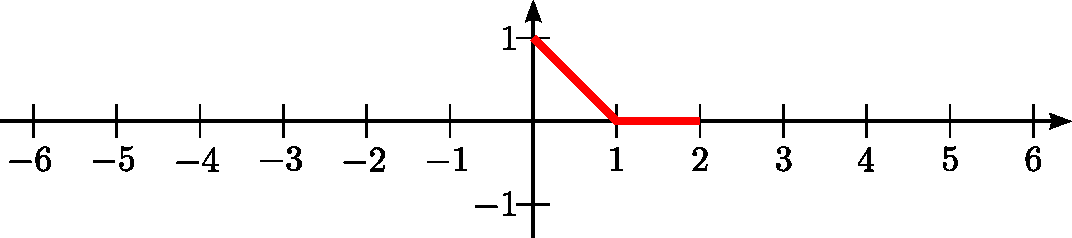
\includegraphics[width=1\textwidth]{fourier0.pdf}
\end{figure}

b)\\
Die Funktion soll zu einer ungeraden Funktion mit Periodenlänge 4 fortgesetzt werden. Machen Sie davon eine Skizze im Bereich $-6 \leq x \leq 6$.\\\\
\begin{figure}[h!]
\centering
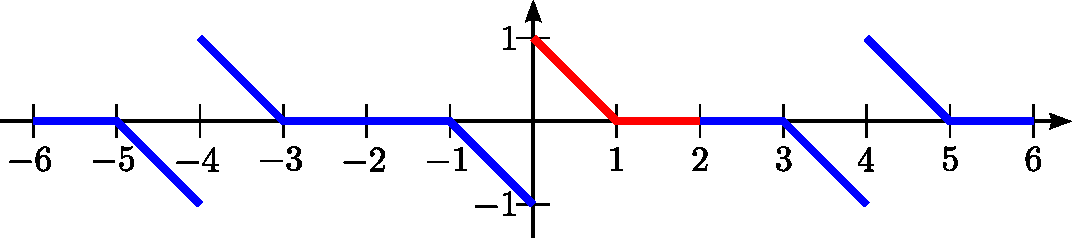
\includegraphics[width=1\textwidth]{fourier1.pdf}
\end{figure}

c)\\
Berechnen Sie die Koeffzienten $a_n$ und $b_n$ der Fourier Reihe dieser periodischen Funktion in allgemeiner Form.


d)\\
Berechnen Sie die Fourierkoeffzienten in numerischer Form (2. St. n. d.
Komma) und schreiben Sie die Fourier Reihe bis und mit der 4. Oberschwingung (Kreisfrequenz $4\omega$) auf.